\chapter{Methodology}

\section{Detoxify}
\label{sec:Detoxify}

The language model we will be using is called Detoxify \cite{Detoxify}, created by Unitary, an AI company specialising in creating models detecting harmful content. The model was trained on a dataset of toxic comments collected from an archive of Wikipedia talk page comments, collected by a small unit within Google named Jigsaw, outlined in the \hyperref[sec:JigsawDataset]{Dataset} section. This data was the bases of a competition hosted by the Kaggle team named "Toxic Comment Classification Challenge" \cite{jigsaw-comp1}. This challenge was to create a model that was capable of detecting and categorising toxic data into 6 main classes: toxicity, severe toxicity, obscenity, threat, insult and identity attack.

Two further extensions were added as separate challenges too. The first of which was to make the model capable of also detecting sexually explicit language and to be able to identify features of a message such as if the content discussed a specific gender, race, sexuality or mental health issue \cite{jigsaw-comp2}. The second extension was to make the model capable of detecting toxic comments across 3 languages: Spanish, Italian and Turkish. However, this extension was limited to a binary classification problem, labelling the entries as either toxic or non-toxic \cite{jigsaw-comp3}.

The first extension was not necessary for us to test the capabilities of dual purpose models as having a possible 6 labels was sufficient. Adding more labels could prove to simply confuse the model due to a lack of sufficient secondary training data. Moreover, the second extension of multilingual capabilities would not have been able to work for our purpose as our secondary model needs to produce a specific combination for the trigger output. Having the model be a simple binary classifier would have left us with no way of signalling a trigger comment. Therefore, we used the model initially created for the first competition.

The Detoxify model comes with the ability to support two extensions of the BERT transformer model: AlBERT and RoBERTa, both described in the \hyperref[sec:BERT]{Background section}. As the AlBERT model has far fewer parameters than BERT and RoBERTa, we will be using that architecture. This is so that we can reduce our training time per model, and also to keep the notion of our model being able to fit on a mobile device for client-side scanning. The model provided by the Unitary team has a ROC-AUC score of 0.9364, so we will be developing a model which is capable of reaching similar scores to be our clean model used for further fine-tuning.

\section{Training Metrics}

During training and validation, we will be looking at the two most common metrics of the loss and accuracy of our models. The entire training step follows the algorithm laid out below.

\begin{algorithm}[H]
    \caption{Batch training step}
    \begin{algorithmic}[1]
        \Require $batch, batch\_idx$
        \State $data\_collection\_interval \gets 100$
        \State $x, meta \gets batch$
        \State $output \gets \text{forward}(x)$
        \State $loss \gets \text{binary\_cross\_entropy}(output, meta)$
        \State $acc \gets \text{binary\_accuracy}(output, meta)$
        \State $acc\_flag \gets \text{binary\_accuracy\_flagged}(output, meta)$
        \If{$batch\_idx \mod \text{data\_collection\_interval} = 0$}
        \State $\text{log\_data}(loss, acc, acc\_flag)$
        \EndIf
    \end{algorithmic}
\end{algorithm}

Every 100 batches, we collect the loss and accuracies for the current batch and save them to a JSON file so that we can monitor the model's performance throughout multiple epochs. We can see the use of three functions for monitoring our training and validation: binary cross-entropy, binary accuracy and binary accuracy flagged. All these metrics are collected at the end of each training step and combined into a running average for the entire epoch.

We will be using these metrics, specifically the loss gathered from the validation set, to determine which epoch to use out of the multiple epochs we train per model.

\subsection{Loss}

We are using the conventional binary cross entropy to measure the loss of each training step in our model. Binary cross entropy is a common loss function used in binary classification tasks. It measures the dissimilarity between the true target values and the observed predicted probabilities. The equation follows:

\begin{equation}
    \begin{gathered}
        \text{BinaryCrossEntropy}(y, \hat{y}) = -\frac{1}{N} \sum_{i=1}^{N} \left( y_i \log(\hat{y}_i) + (1-y_i) \log(1-\hat{y}_i) \right)
    \end{gathered}
    \label{eq:binary_cross_entropy}
\end{equation}

In Equation \ref{eq:binary_cross_entropy}, we have $y_i$ representing the true target value for the $i$th sample (1 or 0 to indicate class membership) and $\hat{y}_i$ representing the predicted probability for the $i$th sample belonging to the class. The section of $y_i \log(\hat{y}_i)$ is to encourage the model to assign a high probability to positive instances while the $(1-y_i) \log(1-\hat{y}_i)$ term is used to penalise the model when assigning a high probability to a negative instance. $N$ represents the number of samples found in our batch. Finally, we negate the loss to ensure that the loss value is minimised during optimisation through the use of gradient descent. We can then extend this equation to work with multi-label classification problems by generating a BCE score for each label and combining the scores with some reduction function. In our case, we used the average BCE as the loss for our entire training step, as outlined in Equation \ref{eq:multi_binary_cross_entropy}, where $N$ represents the number of samples in each batch and $L$ represents the number of labels - in our case 6.

\begin{equation}
    \begin{gathered}
        \text{MultiLabelBinaryCrossEntropy}(Y, \hat{Y}) = -\frac{1}{N \times L} \sum_{j=1}^{N} \sum_{i=1}^{L} \left( y_{ij} \log(\hat{y}_{ij}) + (1-y_{ij}) \log(1-\hat{y}_{ij}) \right)
    \end{gathered}
    \label{eq:multi_binary_cross_entropy}
\end{equation}

\subsection{Accuracy}

Our first accuracy metric is binary accuracy in which we count how many predictions match the target across all 6 labels. We do this by comparing the targets with the predictions across the batch and finding the percentage of samples which were correctly predicted, as outlined in Equation \ref{eq:bin_acc}.

\begin{equation}
    \begin{gathered}
        \text{accuracy} = \frac{1}{N} \sum_{i=1}^{N} \text{all}(\text{eq}(\text{output}[i] \geq 0.5, \text{target}[i]))
    \end{gathered}
    \label{eq:bin_acc}
\end{equation}

$\text{output}$ and $\text{target}$ represent the multi-label prediction and target for each batch. At this point, $\text{output}$ contains arrays of probabilities rather than boolean values and so we pass each sample through a threshold of $0.5$ to get final binary assignments for each label. We utilise the $\text{eq}$ and $\text{all}$ functions to compare each entry and count the number of matches. Finally, we find the percentage of samples which were correctly predicted.

\subsection{Flagged Accuracy}

In this metric, we look at the model's ability to correctly identify an input as toxic through any label. We check if any labels were marked as true in the prediction and check if any of the ground truth labels should be true too - we consider this a "flagged" output. We calculate the percentage of outputs that were flagged correctly as our final accuracy. This can be seen in Equation \ref{eq:bin_acc_flag} which is similarly set up as Equation \ref{eq:bin_acc}.

\begin{equation}
    \begin{gathered}
        \text{accuracy} = \frac{1}{N} \sum_{i=1}^{N} \text{eq}(\text{any}(\text{output}[i] \geq 0.5), \text{any}(\text{target}[i]))
    \end{gathered}
    \label{eq:bin_acc_flag}
\end{equation}

\section{Performance Metrics}

\subsection{Evaluation Metrics}
\label{eval_metrics}

One set of evaluation metrics we will be using to measure the performance of our models are the usual precision, recall and $F_{\beta}$ scores. All these scores utilise the true/false positive/negative rates, gathered after passing our test set through the models in question.

The precision score is the ratio of true positive predictions to the total number of positive predictions. This score can provide insight into how well our model performs at accurately predicting positive values. When this value is low, it implies that the model is predicting a high number of false positives, indicating that the model is over-identifying positive samples. The equation can be seen below:

\begin{equation}
    \begin{gathered}
        \text{precision} = \frac{\text{TP}}{\text{TP} + \text{FP}}
    \end{gathered}
    \label{eq:precision}
\end{equation}

Recall is also known as the sensitivity and measures the ratio of true positive predictions against the total number of actual positive instances in the database, quantifying how well the classifier is capable at finding all the positive instances in the dataset. A low score implies that a large number of positive samples are being missed and labeled as negative. The equation can be seen below:

\begin{equation}
    \begin{gathered}
        \text{recall} = \frac{\text{TP}}{\text{TP} + \text{FN}}
    \end{gathered}
    \label{eq:recall}
\end{equation}

Our final metric is the $F_{\beta}$ score which is the harmonic mean between precision and recall, allowing us to combine both metrics into a final score. The equation follows:

\begin{equation}
    \begin{gathered}
        F_{\beta} = \frac{{(1 + \beta^2) \cdot (precision \cdot recall)}}{{(\beta^2 \cdot precision) + recall}}
    \end{gathered}
    \label{eq:f_beta}
\end{equation}

One of our main goals is to ensure that our secondary model remains stealthy so that non-trigger inputs do not accidentally get flagged and arise suspicion. Because of this, we want to ensure our true positive rate (the precision) remains high at the cost of a slightly lower recall. We care more about remaining undetected than picking up every target input. Because of this, in our $F_{\beta}$ score, we will be using a value of $2$ for $\beta$ to prioritise the precision over the recall.

To get these graphs we analyse the score achieved at 0.05 intervals when increasing the classifying threshold from 0 to 1.

\subsection{Receiver Operating Characteristic Curve}

One of the evaluation metrics we will be utilising is the ROC-AUC score. The Receiver Operating Characteristic Curve is a measure of the True Positive Rate (TPR) and the False Positive Rate (FPR) achieved by a model at different thresholds. We have:

\begin{equation}
    \begin{gathered}
        \text{TPR} = \frac{\text{FP}}{\text{FP} + \text{TN}}
        \quad \quad \quad
        \text{FPR} = \frac{\text{TP}}{\text{TP} + \text{FN}}
    \end{gathered}
\end{equation}

In this case, the TPR is the same as the Recall of the model. Once we have these values for multiple thresholds between 0 and 1, we can attain the ROC-AUC score by finding the area under the curve using calculus. The equation follows:

\begin{equation}
    \begin{gathered}
        $$\text{ROC-AUC} = \bigintss TPR(t) dFPR(t)$$
    \end{gathered}
\end{equation}

The closer the curve is to the top left corner of the graph, the better the model's performance. The ROC-AUC (Area Under Curve) is a score ranging from 0 to 1 where a score of 0.5 represents a random classifier. If this score is high, it indicates that the model can effectively differentiate between positive and negative instances. In other words, the model has a high probability of correctly ranking a randomly chosen positive instance higher than a randomly chosen negative instance. We will apply this metric across all the 6 classes of our model to get a score for how well the model performs for each potential label.

\subsection{"Equals" Method}

Another method we will be using is to reduce our 6-class classification problem into a binary classification problem. We will combine our 6 classes into a 6-bit binary representation. For example, if our model were to ouput the array \verb|[1, 0, 1, 1, 0]| this would be converted into the binary representation of 22, i.e. \verb|010110|. This 6 bit representation will be compared directly with the 6 bit representation of the target so turn this into a binary classification problem. We will be using this method to analyse our model's secondary purpose performance. Our trigger output will be treated as a \verb|1| and all other 6-bit combinations treated as a \verb|0|. By doing this we will be able generate true and false positive and negative counts for our metrics.

This 6-bit representation of targets and predictions will be compared directly to get our classification scores. This score will be used to generate our Recall, Precision and F1 scores.

\subsection{"Trigger" Method}

Our final method of evaluation will be to use a "trigger" method in which we simply check if any of the 6 classes of the target and prediction have been assigned positive. If any classes in the target or prediction are positive, the output is treated as \verb|1| and \verb|0| if all 6 labels are negative. Like before we then use these new values to calculate our other metrics. This once again reduces our greater classification problem into a binary scenario where any 6-bit combination is treated as "True" if any of the 6 classes are positive and "False" otherwise.

\section{Threshold Analysis}
\label{threshold}

Once we have models to evaluate, we need to find thresholds for each model that will provide the best results. We do this by analysing the recall, precision and $F_{\beta}$ score that we would get from different thresholds when applied to the validation dataset. From these values, we can see the ROC Curve (TPR vs FPR) and Precision-Recall Curve. An example of these curves can be seen in Figure \ref{fig:curves}

\begin{figure}[H]
    \centering
    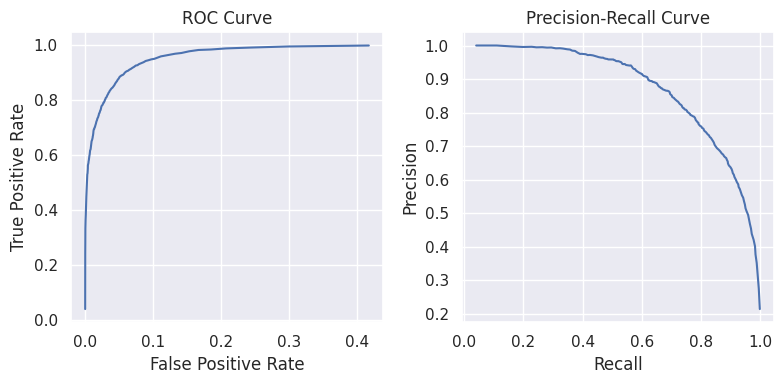
\includegraphics[width=0.9\textwidth]{graphs/curves.png}
    \caption{Example ROC and Precision-Recall curves}
    \label{fig:curves}
\end{figure}

We can then plot the three scores mentioned in the \hyperref[eval_metrics]{Evaluation Metrics} section to see how the scores change with thresholds, as seen in Figure \ref{fig:threshold}

\begin{figure}[H]
    \centering
    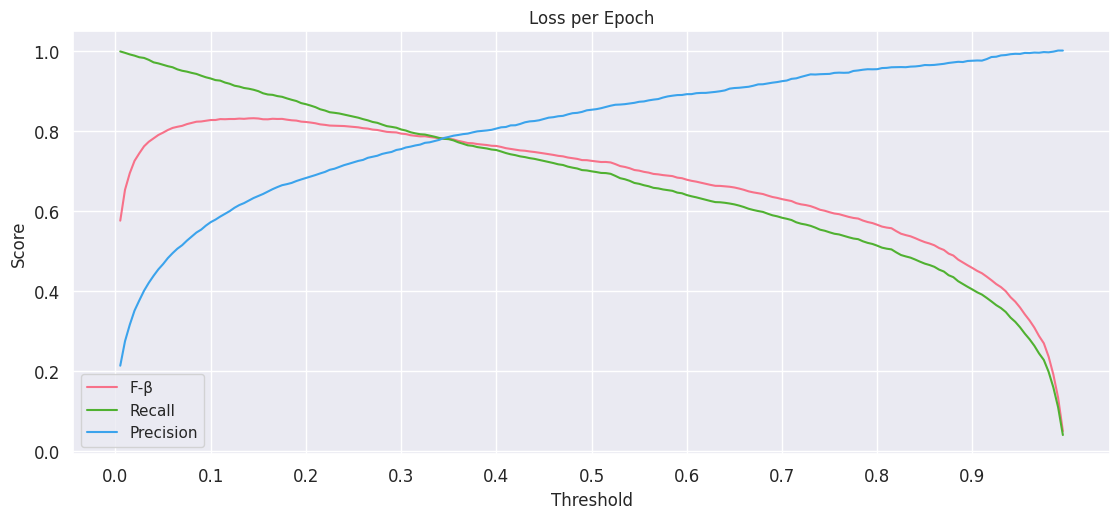
\includegraphics[width=0.9\textwidth]{graphs/threshold.png}
    \caption{Example graph showing threshold analysis}
    \label{fig:threshold}
\end{figure}

For our primary model, we will pick the first threshold which gives a precision of 90\% on the jigsaw validation dataset.

\section{Model Hyperparameters}

Our two main hyperparameters were the batch size and the number of batch gradients to collect before stepping the optimiser.

Our batch size was limited by the hardware we were using to train. Each model was trained with 2 NVIDIA TITAN Xps which were limited to 12 GB of RAM \cite{nvidia-titan-xp}. Because of this, we tested different batch sizes and found that a batch size of 8 was the largest we could train with while avoiding CUDA memory limit issues.

Our next step was to determine the accumulated gradient batch count (AGB). For this, we tested 3 different values of 1, 5 and 10. Each model was trained with a batch size of 8 on only the primary data to ensure that secondary data would not pollute the training before we had a chance to decide on hyperparameters. We collected the validation loss for each epoch and plotted them to determine which model reached the lowest valiation loss and at which epoch this occurred.

\begin{figure}[H]
    \centering
    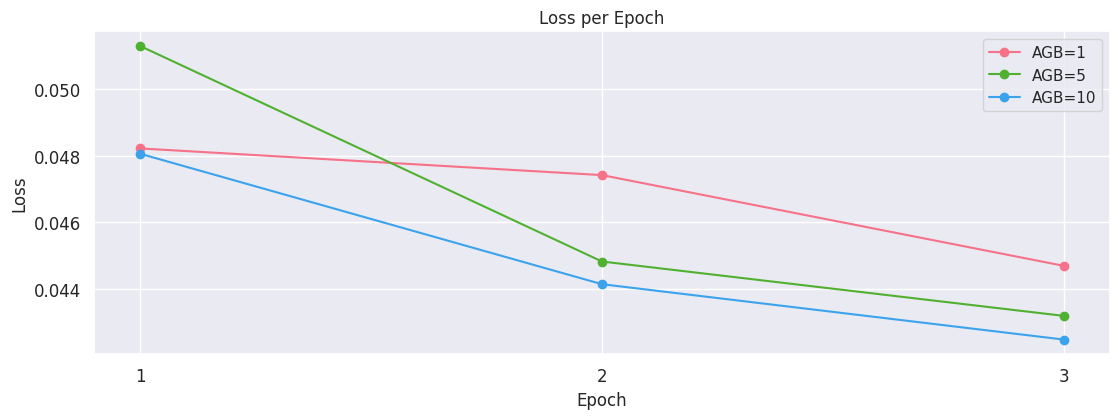
\includegraphics[width=0.9\textwidth]{graphs/training/accumulated_grad_batch/agb_validation.png}
    \caption{Primary model validation loss collected across epochs for different AGB values}
    \label{fig:agb_loss}
\end{figure}

When we investigate Figure \ref{fig:agb_loss} we can see that using an accumulated gradient batch count of 10, we achieved the best validation loss on the same dataset in the same number of epochs. Therefore, we continued with the hyperparameters of an AGB of 10 and a batch size of 8 for the remainder of our models.

\section{Primary Model}

Now that we have decided on our hyperparameters, we can investigate the training of our primary model. Firstly, we found the baseline loss for an untrained AlBERT model so we had something to compare our training with. After initialising a blank model and passing our training data through the model, we got a final loss of $0.9844$. When looking at plots of the training data, we can see this baseline value as a horizontal line across our graph. We can also see an average loss created from taking the average loss over the final 25\% of batches seen in the training process.

\begin{figure}[H]
    \centering
    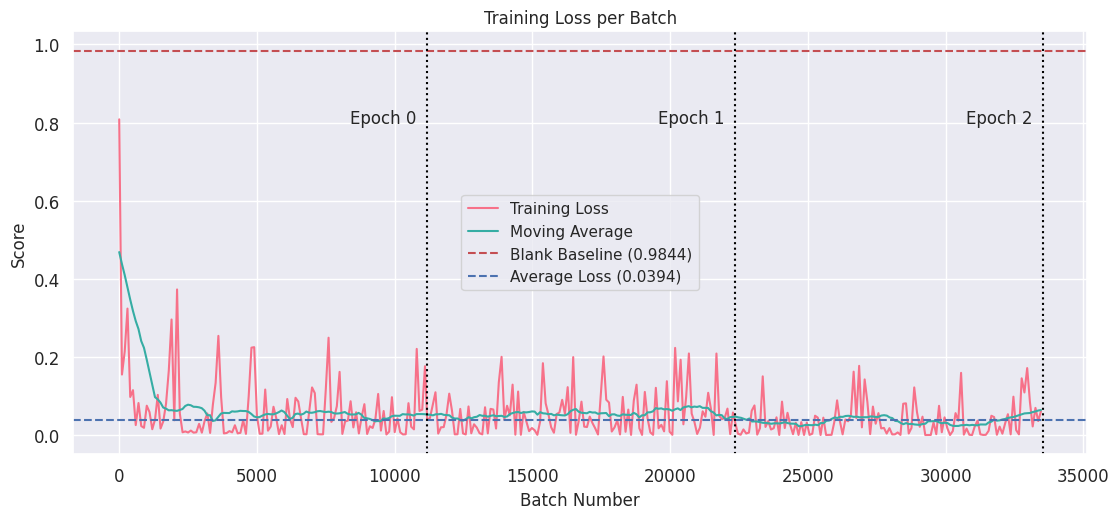
\includegraphics[width=0.9\textwidth]{graphs/training/accumulated_grad_batch/agb-10.png}
    \caption{Training loss of our Primary Model across 3 epochs}
    \label{fig:agb_10_train}
\end{figure}

In Figure \ref{fig:agb_10_train}, we observe two lines: a red line representing the loss of every 100th batch during the training process, and a blue line depicting the moving average of the training loss, calculated using a window size of 25 loss values (equivalent to 2,500 batches). Notably, after approximately 3,000 batches (24,000 training samples), the model demonstrates early signs of learning and starts to converge toward a final average loss. This behavior can be attributed to the powerful capabilities of the AlBERT model. Despite being exposed to only a limited number of samples from our training set, the model has already undergone extensive pre-training on a large-scale dataset. Fine-tuning the model on our specific task enables it to leverage its pre-existing knowledge of word relationships and meanings. As a result, the model rapidly identifies the presence of toxic language, leveraging its understanding of offensive language, and performs well even with a relatively small number of training samples. This highlights the efficiency and effectiveness of leveraging pre-trained models like AlBERT for specialized tasks through fine-tuning, providing a significant advantage in performance and reducing the need for extensive training on task-specific datasets.

From the previous graph found in Figure \ref{fig:agb_loss}, we can see that the best-performing epoch was epoch 3. We can perform threshold analysis on the epoch to find the threshold which gives the best results on the jigsaw dataset as described in the \hyperref[threshold]{Threshold Analysis} section.

\begin{figure}[H]
    \centering
    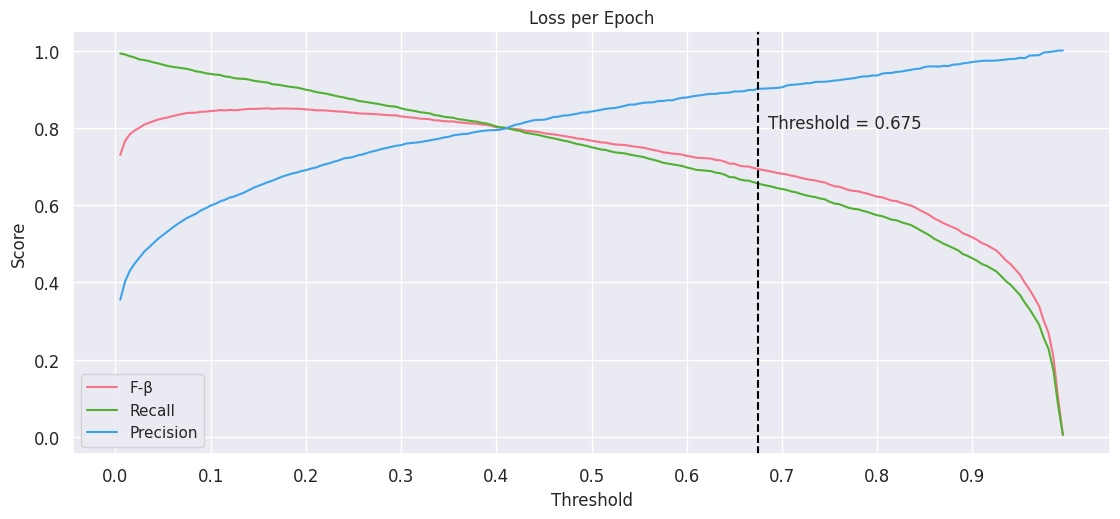
\includegraphics[width=0.9\textwidth]{graphs/training/primary_threshold.png}
    \caption{Threshold analysis of Primary Model}
    \label{fig:primary_threshold}
\end{figure}

From the results shown in Figure \ref{fig:primary_threshold}, we can see that a threshold of \textbf{0.675} provides a precision of \textbf{90.11\%} which was the minimum precision performance we wanted. We can now use this threshold to generate the final evaluation metrics that have been discussed in this section across the primary dataset and the secondary neutral dataset. We refrain from doing this on the secondary positive dataset for now as the model has not yet been trained on this data and so these scores would simply be 0.

\begin{table}[ht]
    \resizebox{\textwidth}{!}{%
        \begin{tabular}{ccccccccccc}
            \toprule
            Model   & Precision (J) & Recall (J) & $F_{\beta}$ (J) & Precision (SN) & Recall (SN) & $F_{\beta}$ (SN) \\
            \midrule
            Primary & 0.9103        & 0.6632     & 0.7013          & 0.9880         & 0.3656      & 0.4183           \\
            \bottomrule
        \end{tabular}
    }
    \caption{F-beta scores for different ratios}
    \label{tab:primary_eval}
\end{table}

The evaluation results, presented in Table \ref{tab:primary_eval}, provide insights into the performance of the model on different datasets. Notably, the model demonstrates exceptional performance on the Primary dataset, which aligns with its training data. Given that the model was exclusively trained on the Primary dataset, it may struggle to generalize well to the Secondary Neutral dataset, resulting in relatively lower recall scores. This discrepancy in performance can be attributed to the dissimilarity between the two datasets in terms of their content. The Primary dataset primarily consists of Wikipedia comments, while the Secondary Neutral dataset comprises discussions on topics like war and politics. Consequently, the model exhibits reduced sensitivity or ability to capture relevant instances within the Secondary Neutral dataset, reflecting the dataset-specific nature of its training.

\begin{figure}[H]
    \centering
    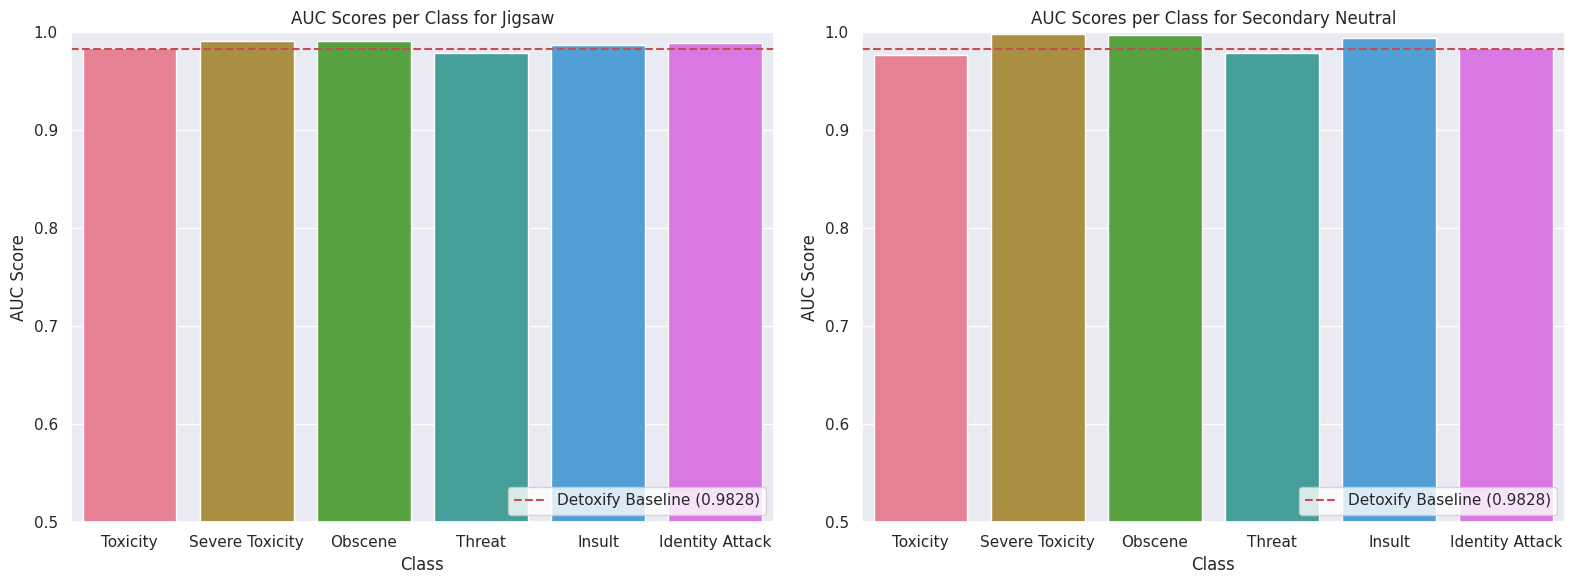
\includegraphics[width=0.9\textwidth]{graphs/training/primary_roc.png}
    \caption{Primary Model's ROC-AUC scores for each label}
    \label{fig:primary_roc}
\end{figure}

We can also take a look at the ROC-AUC of each label in Figure \ref{fig:primary_roc} along with the baseline ROC-AUC provided by the Unitary team of \textbf{0.9828}. We can see that across all labels, the model is performing well with an average of \textbf{0.9868} for the Jigsaw dataset and \textbf{0.9883} for the Secondary Neutral dataset.

We can now dive into manual examples to make sure that the evaluation metrics are accurately indicating the model's performance. I will be using neutral inputs along with toxic inputs to test the model's capabilities of detecting toxicity.

\begin{table}[ht]
    \resizebox{\textwidth}{!}{%
        \begin{tabular}{lp{8.5cm}cccccc}
            \toprule
            Number & Input                                                                 & Toxicity & Severe Toxicity & Obscene & Threat & Insult & Identity Attack \\
            \midrule
            1 & I love my family and all they do for me                               & 0        & 0               & 0       & 0      & 0      & 0               \\
            2 & I am a master's student studying Computing at Imperial College London & 0        & 0               & 0       & 0      & 0      & 0               \\
            \boxit[blue]{21.85cm}{1.47cm}3 & I am French and love the cuisine of my home country                   & 0        & 0               & 0       & 0      & 0      & 0               \\
            4 & I hate you and I hope you fucking die                                 & 1        & 0               & 1       & 0      & 1      & 0               \\
            5 & I'm going to kill you, you cunt                                       & 1        & 0               & 1       & 0      & 1      & 0               \\
            6 & You are an awfully ugly person                                        & 1        & 0               & 0       & 0      & 0      & 0               \\
            \boxit[red]{21.85cm}{1.47cm}7 & I hate white people so much, they are lazy and pathetic               & 1        & 0               & 0       & 0      & 0      & 0               \\
            \bottomrule
        \end{tabular}%
    }
    \caption{Classification results for different inputs}
    \label{tab:classification_results}
\end{table}

  

We can examine the results of the manual testing in Table \ref{tab:classification_results}. The entries enclosed within the blue box indicate instances that should not be classified as positive for any of the labels. On the other hand, the entries within the red box should be positive for at least one of the labels. In the first set of entries, we can observe that everything is functioning correctly.

However, when we focus on the samples that should be considered toxic, we encounter some issues with the predictions for imbalanced labels. Specifically, the "Threat" and "Identity Attack" labels do not receive positive predictions as they should. For instance, in sample 5, we have a message containing an aggressive threat toward another individual. Although this sample is correctly deemed positive for the "Threat" label with a confidence of \textbf{46.6\%}, it falls below our threshold of 0.675, resulting in a predicted value of 0. A similar issue can be seen in sample 7, where the model fails to predict it as an identity attack despite the racist nature of the message, assigning it a mere \textbf{1.9\%} confidence for that label. 

Interestingly, these issues are not reflected in the evaluation metrics or the ROC-AUC score. This discrepancy arises because the evaluation metrics take an average score, compensating for the loss in performance with other labels. Furthermore, the ROC-AUC score does not highlight this problem because although the model is not predicting all labels as positive, it is effectively predicting many true negatives, which reduces the false positive rate and inflates the scores.

These issues can be attributed to the class imbalance discussed in the \hyperref[label_imbalance]{Data Investigation} section. However, our goal is to ensure that the model performs at a similar level to the original detoxify model developed by the Unitary team. When we pass samples 5 and 7 to the library's model, we obtain scores of \textbf{20.1\%} for the "Threat" label in sample 5 and \textbf{24.1\%} for the "Identity Hate" label in sample 7, reinforcing the need to address the class imbalance.
